\section{The Memory Problem}\label{sec:mem_problem}
It is worthwhile to discuss the memory usage of the algorithm as the program unfolds. For arguments sake, let us use the attribute values from the discussion in section \ref{sec:degOfPar}, that is, let the grid be 3000 by 3000 pixels and both the amount of lines per scan and the amount of angle increments be 2000. As mentioned previously, an array with an entry for each pixel in the grid is constructed for each line. Assuming that each entry in this array is encoded as a 32-bit floating point value, then the space occupies in memory by each array is:
$$3000^2 \cdot 32~\text{bit} = 288,000,000 ~\text{bit} = 72 ~\text{mb}$$ 
Multiply that by the total amount of lines and we arrive at a total memory usage of 
$$72 ~\text{mb} \cdot 2000^2 = 288,000,000~\text{mb} = 288~\text{tb}$$ 
An internet search reveals that a typical GPU has about 8-12 gb of memory, at the time of this project, so obviously this amount of data is way beyond what is suitable for current GPUs (or a consumer hard-drive for that matter). 
All is not lost however, as there are methods to reduce the memory usage. First let us have a look at how well we utilize the memory we've allocated for the line result arrays.
Initially a result array is filled with $-1$ and then the pixels that the particular line intersects is updated with the intersection lengths. This means that the array is mostly filled with $-1$, it is therefore said to be a \emph{sparse} matrix. We know from \cite{FCT} that the amount of non-negative values of a given line is at most $2 \cdot gridsize - 1$, but often less. Using this we can compute the \emph{density} of the most dense matrix. We have that 
$$\text{maximal density} = \frac{(2 \cdot gridsize - 1)}{gridsize^2}$$
Plotting the maximal density as a function of the grid size produces the following graph:
\begin{figure}[H]
  \centering
  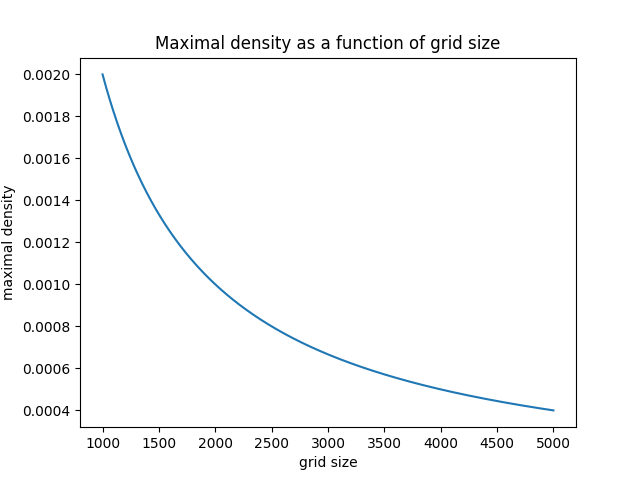
\includegraphics[scale=0.8]{figures/maxdensity.png}
  \caption{Maximal density as a function of grid size.}
\end{figure}

We note that with a grid size between 1000 and 5000 the density seems to vary from $~\sim 0.002$ down to $~\sim 0.0005$.
In the example presented above, we have a maximal density of $\frac{(2 \cdot 3000 - 1)}{3000^2} = 0.0006$, meaning that only $0.06\%$ of the entries in the array actually contain interesting values, the rest are $-1$. 
This is an abysmal utilization of the memory we've allocated. In the next section we will describe a method of compression to improve on this issue.

\subsection{Compressing Our Matrices}
All methods of compressing sparse matrices use some sort of strategy to save meaningful values along with their position in the original matrix. With respect to implementation the simplest method is to save an array of values and their 2D-index pairs. A slightly modified approach was taken in this project: We save an array of pairs containing values and flat indices. Given an original position in a matrix, $(i, j)$, and a grid size $g$, then the flat index $k$ is $k = g \cdot i + j$. This lets us save one less integer per entry.

There is a caveat though: Since there can be a different amount of intersected pixels from one line to another, the arrays that result from our compression can have irregular lengths. For parallelization Futhark requires that each kernel uses the same amount of memory, so we need to fix the length of our compressed matrices. Fortunately we know from \cite{FCT} that one line can have at most $2 \cdot g - 1$ intersected pixels. This means that we can allocate $2 \cdot g - 1$ pairs of sentinel values, say $(-1,~-1)$, and update them with the actual values as the algorithm finds them. The total amount of memory for one line is then given by:
$$2 \cdot (2 \cdot g - 1) \cdot 32~\text{bit}$$
Using the example from earlier, with a grid size of 3000 by 3000 and line- and angle-counts at 2000, we get the following memory usage per line:
$$2 \cdot (2 \cdot g - 1) \cdot 32~\text{bit} = 383,936~\text{bit} = ~\sim 48~\text{kb}$$ 
And in total we use: 
$$383,936~\text{bit} \cdot 2000^2 = 1,535,744,000,000~\text{bit} = ~\sim 192~\text{gb}$$
This is an improvement in memory usage of roughly $\frac{288000}{192}\cdot100 = 150,000\%$. But maybe even more importantly we now scale linearly in memory usage with grid size rather than quadratically.

We deem this method of compression very viable, but that is not to say that there are no further improvements to be made in this area. In section \ref{sec:CRS} we describe another compression method called \emph{Compressed Row Matrices}. These have a little less memory usage but more importantly they feature some desirable attributes related to matrix-vector multiplications, which are widely used in ART. The reason for not using this method (yet) in this project is that it proved difficult to implement in Futhark (it inherently includes some irregular arrays).